\chapter{Relazioni}
In generale, siano dati gli insiemi $A, B$ e $AxB$. Come sappiamo, ad $AxB$ appartengono tutte le coppie costituite da un primo elemento tratto da $A$ e da un secondo elemento tratto da $B$. Ogni sottoinsieme di $AxB$ potrà essere considerato come una relazione tra gli elementi di $A$ e quelli di $B$. 

\begin{definition}[Relazione]
    Si dice relazione (o corrispondenza) tra gli insiemi $A$ e $B$ un sottoinsieme del prodotto cartesiano $AxB$.
\end{definition}

Ad esempio consideriamo gli insiemi $A = \{Arno, Po, Tevere\}$ e \\$B = \{Firenze, Pisa, Torino\}$, e il loro prodotto cartesiano, formato da tutte le coppie aventi per primo elemento un un fiume e per secondo un elemento una città. Individuiamo quelle costituite dal nome di un fiume e da quello di una città bagnata da tale fiume: $R = \{(Arno, Firenze), (Arno, Pisa), (Po, Torino)\}\\R\subseteq AxB$.

Una relazione, come ogni sottoinsieme del prodotto cartesiano di insiemi, può spesso essere rappresentata graficamente. Il precedente esempio può essere rappresentato dalla seguente tabella:
\begin{center}
\begin{tabular}{c|c|c|c}
     & Arno & Po & Tevere\\\hline
     Torino & & \checkmark  &\\\hline
     Pisa & \checkmark & &\\\hline
     Firenze & \checkmark & &
\end{tabular}
\end{center}

\section{Relazioni tra un insieme e se stesso}
Per definizione del prodotto cartesiano di due insiemi, non è necessario che gli insiemi in questione siano distinti: come abbiamo visto, è possibile parlare del prodotto cartesiano $IxI$, costituito dall’insieme di tutte le coppie ordinate $(a, b)$ con $a\in I$ e $b \in I$. Esamineremo ora le caratteristiche delle relazioni definite in $IxI$; tali relazioni possono infatti godere di interessanti proprietà, introdotte dalle definizioni seguenti.

\begin{definition}[Riflessiva]
    Si dice che la relazione $R\subseteq IxI$ gode della proprietà riflessiva se, $\forall a\in I, (a, a)\in R$.
\end{definition} 
Cioè se ogni elemento dell’insieme considerato è in relazione con se stesso.

\begin{definition}[Antiriflessiva]
    Si dice che la relazione $R\subseteq IxI$ gode della proprietà antiriflessiva se, $\forall a\in I, (a, a)\notin R$.
\end{definition}
Cioè se nessun elemento dell’insieme considerato è in relazione con se stesso.

\begin{definition}[Simmetrica]
    Si dice che la relazione $R\subseteq IxI$ gode della proprietà simmetrica se, $\forall a,b\in I$, si ha che, se $(a, b)\in R$, allora $(b, a)\in R$.
\end{definition}
Cioè quando per ogni coppia di elementi a e b dell’insieme considerato, accade che, se a è in relazione con b, allora anche b è in relazione con a.

\begin{definition}[Antisimmetrica]
    Si dice che la relazione $R\subseteq IxI$ gode della proprietà antisimmetrica se, $\forall a,b\in I$, si ha che, se $(a, b)\in R$ e $(b, a)\in R$, allora $a = b$.
\end{definition}
Cioè quando per ogni coppia di elementi a e b dell’insieme considerato, il contemporaneo essere a in relazione con b e b in relazione con a implica che $a = b$.

\begin{definition}
    Si dice che la relazione $R\subseteq IxI$ gode della proprietà transitiva se, $\forall a,b,c\in I$, si ha che, se $(a, b)\in R$ e $(b, c)\in R$, allora $(a, c)\in R$.
\end{definition}
Cioè quando, per ogni terna di elementi a, b e c dell’insieme considerato, accade che, se a è in relazione con b e b è in relazione con c, allora a è in relazione con c.

\begin{example}
    Consideriamo nell’insieme $I$ delle rette del piano la $R\subseteq IxI$ tale che $R = \{(r, s): r$ è coincidente o parallela a $s\}$. Tale relazione gode delle proprietà: 
    \begin{enumerate}
        \item Riflessiva, perché ogni retta è coincidente o parallela a se stessa (nel caso specifico, coincidente);
        \item Simmetrica, perché se la retta $r$ è coincidente o parallela alla retta $s$, allora anche $s$ è coincidente o parallela a $r$;
        \item Transitiva, perché se la retta $r$ è coincidente o parallela alla retta $s$ e la retta $s$ è coincidente o parallela alla retta $t$, allora la retta $r$ risulta coincidente o parallela a $t$.
    \end{enumerate}
\end{example}

Data una relazione si può sempre costruire una “minima” relazione transitiva che la contenga come insieme. Denoteremo questo rapporto con il termine \textbf{chiusura transitiva}. La relazione transitiva ha quindi la proprietà di essere la più piccola relazione transitiva possibile.
\begin{example}
    $A=\{1,2,3,4\}\hspace{0,5cm}\hat{R}=\{(1,3),(1,4),(4,1),(1,1)(4,4),(4,3)\}$
\end{example}

\section{Relazioni di equivalenza}
\begin{definition}[Relazione di equivalenza]
    Una relazione $R\subseteq IxI$ si dice relazione di equivalenza se gode delle proprietà riflessiva, simmetrica e transitiva.
\end{definition}
\begin{definition}[Classe di equivalenza]
    Si dice classe di equivalenza dell’elemento $a\in I$ il sottoinsieme di $I$ costituito dagli elementi $x$ tali che $(a, x)\in R$; tale insieme verrà denotato con [a].
\end{definition}
Ad esempio una classe di equivalenza può essere rappresentata dai numeri pari o dai numeri dispari dell'insieme $\mathbb{N}$.
\begin{definition}
    Si dice insieme quoziente dell’insieme $I$ l’insieme delle classi di equivalenza degli elementi di $I$ rispetto alla relazione di equivalenza R.
\end{definition}
L’insieme quoziente costituisce una partizione di $I$: con ciò intendiamo che l’insieme quoziente è un insieme di sottoinsiemi di $I$ non vuoti, a due a due disgiunti e la cui l’unione è $I$.

\section{Relazioni d'ordine}
Introduciamo ora un’altra importante classe di relazioni.
\begin{definition}[Ordine largo]
    Una relazione si dice relazione d’ordine largo se gode delle proprietà riflessiva, antisimmetrica e transitiva.    
\end{definition}
\begin{definition}[Ordine stretto]
    Una relazione si dice relazione di ordine stretto se gode delle proprietà antiriflessiva e transitiva.    
\end{definition}
Per capire meglio la differenza si può fare il seguente esempio: 
\begin{example}
    Presi due numeri $a$ e $b$ e conforntati tra loro con $\leq$ e $<$, si nota come una relazione sia di ordine largo, mentre l'altra di ordine stretto.
\end{example}
\begin{definition}[Ordine totale]
    Una relazione d’ordine $S$ definita in un insieme $I$ e tale che, per ogni coppia di elementi $a$ e $b$ si verifica sempre uno dei casi $(a, b)\in S$ oppure $(b, a)\in S$ (ovvero che consenta il confronto di tutte le coppie di elementi di $I$) si dice relazione d’ordine totale.
\end{definition}
\begin{definition}[Ordine parziale]
    Una relazione d’ordine $S$ che non per tutte le coppie consenta tale confronto, ovvero tale che per almeno una coppia di elementi $c$ e $d$ dell’insieme considerato accada che $(c, d)\notin S$ e che $(d, c)\notin S$, si dice relazione d’ordine parziale.
\end{definition}
Infine, notiamo che a volte un insieme ordinato può essere specificato in maniera diagrammatica, collegando con una freccia il primo elemento di ogni coppia della relazione con il rispettivo secondo elemento, come in figura \ref{fig:es_relazion}.
\begin{figure}[ht]
    \centering
    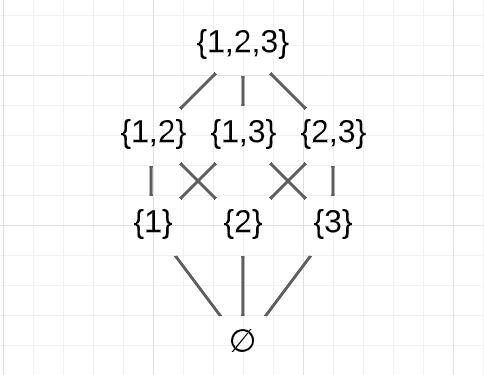
\includegraphics[width = 6cm]{images/es_relazioni.JPG}
    \caption{Insieme dei sottoinsiemi di $\{1, 2, 3\}$, ordinato mediante inclusione insiemistica.}
    \label{fig:es_relazion}
\end{figure}
\begin{definition}
    Dato un insieme $X$ e una relazione d’ordine $\leq$ su di esso, si dice:
    \begin{itemize}
        \item massimo un elemento $x_1:\forall x\in X, x\leq x_1$;
        \item minimo un elemento $x_0:\forall x\in X, x_0\geq x$;
        \item massimo comune minorante tra due elementi $x, y\in X$ e due elementi $z$ e $z'\in X:z$ e $z'$ siano $\leq$ di $x$ e $y$, accade $z \leq z'$;
        \item minimo comune maggiorante tra due elementi $x, y\in X$ e due elementi $t$ e $t'\in X:t$ e $t'$ siano $\geq$ di $x$ e $y$, accade $t' \geq t$.
    \end{itemize}
\end{definition}
\begin{example}
    Si consideri l’insieme dei numeri naturali positivi con la relazione di divisibilità: esiste un minimo (il numero 1), non esiste un massimo, esistono massimo comune minorante e minimo comune maggiorante di due numeri e sono rispettivamente il loro massimo comun divisore (M.C.D.) e minimo comune multiplo (m.c.m.).
\end{example}